\documentclass[table,letterpaper]{beamer}
\usetheme{Warsaw}
\usepackage[utf8]{inputenc}
\usepackage{tabu}
\usepackage{amsmath}
\usepackage{gensymb}
\usepackage{graphicx}

%Information to be included in the title page:
\title{Rotation}
\author{Physics Club}
\date{November 13, 2014}
 
\begin{document}

\frame{\titlepage}

\begin{frame}
\frametitle{Basic Definitions}
\begin{block}{Radian}
Unit of angular measure. By definition, the angle in radians is equal to the length subtended.\\
One radian is approximately 180$\degree$/$\pi = 57.30\degree$.
\end{block}

\begin{block}{Angular Displacement $\Delta \theta$}
$$\Delta s = r\Delta \theta$$
\end{block}

\begin{block}{Angular Velocity $\omega$}
$$v = r\omega$$
\end{block}

\begin{block}{Angular Acceleration $\alpha$}
$$a_t = r\alpha$$
$$a_c = \frac{v^2}{r} = r\omega^2$$
\end{block}
\end{frame}

\begin{frame}
\frametitle{Angular Quantities}
\renewcommand{\arraystretch}{1.5}
\begin{center}
{\tabulinesep=1.2mm
\begin{tabu}{c | c | c}
& Translational & Rotational\\ \hline
Displacement & $\displaystyle \Delta x$ & $\displaystyle \Delta \theta$\\
Velocity & $\displaystyle v$ & $\displaystyle \omega$\\
Acceleration & $\displaystyle a$ & $\displaystyle \alpha$\\
Equation \#1 & $\displaystyle \Delta x = \bar{v}t$ & $\displaystyle \Delta \theta = \bar{\omega}t$\\
Equation \#2 & $\displaystyle v = v_0 + at$ & $\displaystyle \omega = \bar{\omega}t$\\
Equation \#3 & $\displaystyle \Delta x = v_0t + \frac{1}{2}at^2$ & $\displaystyle \Delta \omega = \omega_0t + \frac{1}{2}\alpha t^2$\\
Equation \#4 & $\displaystyle \Delta x = v_0t - \frac{1}{2}at^2$ & $\displaystyle \Delta \omega = \omega_0t - \frac{1}{2}\alpha t^2$\\
Equation \#5 & $\displaystyle v^2 = v_0^2 + 2a\Delta x$ & $\displaystyle \omega^2 = \omega_0^2 + 2\alpha\Delta\theta$\\
\end{tabu}}
\end{center}
\end{frame}

\begin{frame}
\frametitle{The Right-Hand Rule}
\vfill
Angular quantities are vectors. Angular displacement, angular velocity, and angular acceleration are all vectors.\\
\vfill
Use the right-hand rule to find the direction of the angular velocity $\omega$ vector.\\
\vfill
The angular acceleration $\alpha$ vector is the same direction if the angular velocity $\omega$ is increasing with time, opposite if decreasing.
\vfill
\end{frame}

\begin{frame}
\frametitle{Rotational Kinetic Energy \& Moment of Inertia}
\begin{block}{Rotational Kinetic Energy $K$}
$$K = \sum \left(\frac{1}{2}m_iv_i\right) = \frac{1}{2}\sum \left(m_ir_i^2\omega^2\right) = \frac{1}{2}I\omega^2$$
\end{block}

\begin{block}{Moment of Inertia $I$}
$$I = \sum m_ir_i^2$$
\end{block}

\begin{block}{The Parallel-Axis Theorem}
$$I = I_\text{cm} + Mh^2$$
\end{block}
\end{frame}

\begin{frame}
\frametitle{Moments of Inertia}
\begin{center}
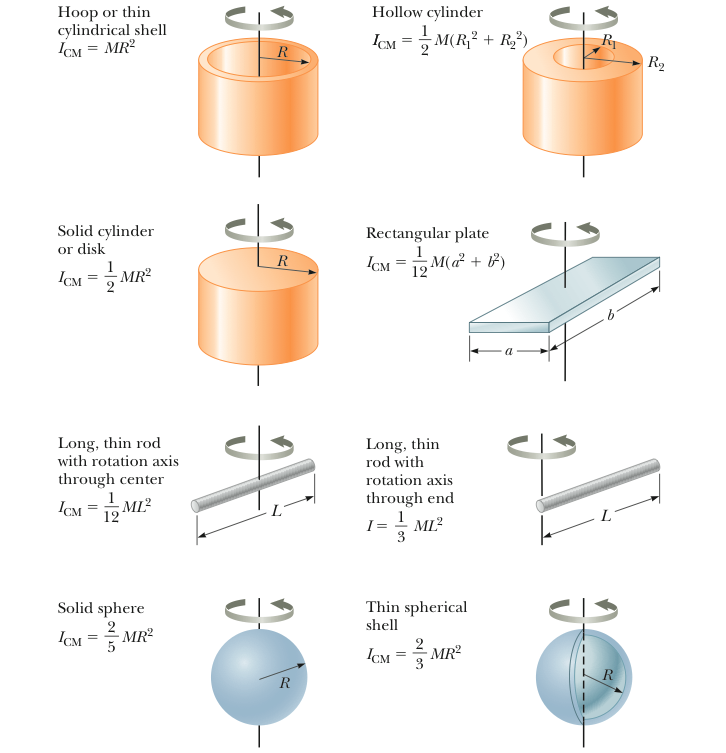
\includegraphics[height=0.9\textheight]{inertia.png}
\end{center}
\end{frame}

\begin{frame}
\frametitle{Newton's Second Law for Rotation}
\begin{block}{Torque $\tau$}
$$\tau = rF_t = rF\sin \phi = F\ell$$
\end{block}

\begin{block}{Work $W$}
$$\Delta W = F_tr\Delta \theta$$
\end{block}

\begin{block}{Newton's Second Law for Rotation}
$$\sum \tau_\text{ext} = I\alpha$$
\end{block}

\begin{block}{Power}
$$P = \frac{\Delta W}{\Delta t} = \frac{\tau\Delta\theta}{\Delta t} = \tau\omega$$
\end{block}
\end{frame}

\begin{frame}
\frametitle{Angular Momentum}
\begin{block}{Angular Momentum $L$}
$$L = I\omega = r \times p$$
\end{block}

\begin{block}{Conservation of Angular Momentum}
$L_\text{sys}$ is constant if the external torque on the system is 0.
\end{block}

\begin{block}{Rolling}
When rigid objects roll, there are two types of basic rolling: ``with slipping'' and ``without slipping''. $$v_\text{cm} = R\omega$$
\end{block}
\end{frame}

\end{document}